%-------------------------
% Resume in Latex
% Author
% License : MIT
%------------------------

%---- Required Packages and Functions ----

\documentclass[a4paper,11pt]{article}
\usepackage{latexsym}
\usepackage{xcolor}
\usepackage{float}
\usepackage{ragged2e}
\usepackage[empty]{fullpage}
\usepackage{wrapfig}
\usepackage{lipsum}
\usepackage{tabularx}
\usepackage{titlesec}
\usepackage{geometry}
\usepackage{marvosym}
\usepackage{verbatim}
\usepackage{enumitem}
\usepackage[hidelinks]{hyperref}
\usepackage{fancyhdr}
\usepackage{fontawesome5}
\usepackage{multicol}
\usepackage{graphicx}
\usepackage{cfr-lm}
\usepackage[T1]{fontenc}
\setlength{\multicolsep}{0pt} 
\pagestyle{fancy}
\fancyhf{} % clear all header and footer fields
\fancyfoot{}
\renewcommand{\headrulewidth}{0pt}
\renewcommand{\footrulewidth}{0pt}
\geometry{left=1.4cm, top=0.8cm, right=1.2cm, bottom=1cm}
% Adjust margins
%\addtolength{\oddsidemargin}{-0.5in}
%\addtolength{\evensidemargin}{-0.5in}
%\addtolength{\textwidth}{1in}
\usepackage[most]{tcolorbox}
\tcbset{
	frame code={}
	center title,
	left=0pt,
	right=0pt,
	top=0pt,
	bottom=0pt,
	colback=gray!20,
	colframe=white,
	width=\dimexpr\textwidth\relax,
	enlarge left by=-2mm,
	boxsep=4pt,
	arc=0pt,outer arc=0pt,
}

\urlstyle{same}

\raggedright
\setlength{\tabcolsep}{0in}

% Sections formatting
\titleformat{\section}{
  \vspace{-4pt}\scshape\raggedright\large
}{}{0em}{}[\color{black}\titlerule \vspace{-7pt}]

%-------------------------
% Custom commands
\newcommand{\resumeItem}[2]{
  \item{
    \textbf{#1}{\hspace{0.5mm}#2 \vspace{-0.5mm}}
  }
}

\newcommand{\resumePOR}[3]{
\vspace{0.5mm}\item
    \begin{tabular*}{0.97\textwidth}[t]{l@{\extracolsep{\fill}}r}
        \textbf{#1}\hspace{0.3mm}#2 & \textit{\small{#3}} 
    \end{tabular*}
    \vspace{-2mm}
}

\newcommand{\resumeSubheading}[4]{
\vspace{0.5mm}\item
    \begin{tabular*}{0.98\textwidth}[t]{l@{\extracolsep{\fill}}r}
        \textbf{#1} & \textit{\footnotesize{#4}} \\
        \textit{\footnotesize{#3}} &  \footnotesize{#2}\\
    \end{tabular*}
    \vspace{-2.4mm}
}

\newcommand{\resumeProject}[4]{
\vspace{0.5mm}\item
    \begin{tabular*}{0.98\textwidth}[t]{l@{\extracolsep{\fill}}r}
        \textbf{#1} & \textit{\footnotesize{#3}} \\
        \footnotesize{\textit{#2}} & \footnotesize{#4}
    \end{tabular*}
    \vspace{-2.4mm}
}

\newcommand{\resumeSubItem}[2]{\resumeItem{#1}{#2}\vspace{-4pt}}

% \renewcommand{\labelitemii}{$\circ$}
\renewcommand{\labelitemi}{$\vcenter{\hbox{\tiny$\bullet$}}$}

\newcommand{\resumeSubHeadingListStart}{\begin{itemize}[leftmargin=*,labelsep=0mm]}
\newcommand{\resumeHeadingSkillStart}{\begin{itemize}[leftmargin=*,itemsep=1.7mm, rightmargin=2ex]}
\newcommand{\resumeItemListStart}{\begin{justify}\begin{itemize}[leftmargin=3ex, rightmargin=2ex, noitemsep,labelsep=1.2mm,itemsep=0mm]\small}

\newcommand{\resumeSubHeadingListEnd}{\end{itemize}\vspace{2mm}}
\newcommand{\resumeHeadingSkillEnd}{\end{itemize}\vspace{-2mm}}
\newcommand{\resumeItemListEnd}{\end{itemize}\end{justify}\vspace{-2mm}}
\newcommand{\cvsection}[1]{%
\vspace{2mm}
\begin{tcolorbox}
    \textbf{\large #1}
\end{tcolorbox}
    \vspace{-4mm}
}

\newcolumntype{L}{>{\raggedright\arraybackslash}X}%
\newcolumntype{R}{>{\raggedleft\arraybackslash}X}%
\newcolumntype{C}{>{\centering\arraybackslash}X}%
%---- End of Packages and Functions ------

%-------------------------------------------
%%%%%%  CV STARTS HERE  %%%%%%%%%%%
%%%%%% DEFINE ELEMENTS HERE %%%%%%%
\newcommand{\name}{Linh Vo Tran Nha} % Your Name
\newcommand{\course}{Computer Engineering} % Your Program
\newcommand{\phone}{0865167913} % Your Phone Number
\newcommand{\emaila}{linh.vo1011@hcmut.edu.vn} %Email 1
\newcommand{\emailb}{vtrnnhlinh@gmail.com} %Email 2
\newcommand{\dob}{10/11/2003} %Date of Birth



\begin{document}
\fontfamily{cmr}\selectfont
%----------HEADING-----------------


\parbox{2.35cm}{%
  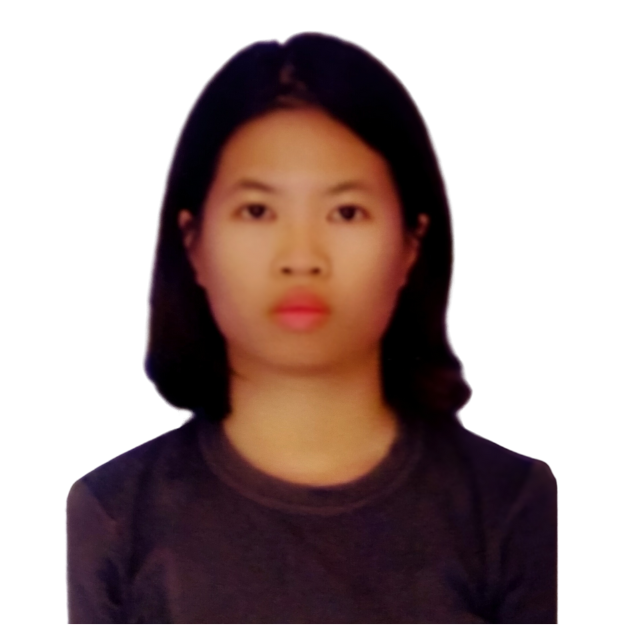
\includegraphics[width=2.35cm,clip]{avatar.png}
}
\parbox{\dimexpr\linewidth-2.8cm\relax}{
  \begin{tabularx}{\linewidth}{L r}                                                                                                                                                   \\
    \textbf{\Large \name}                        & {\raisebox{0.0\height}{\footnotesize \faPhone}\ \phone}                                                              \\
    \dob                                         & \href{mailto:\emailb}{\raisebox{0.0\height}{\footnotesize \faEnvelope}\ {\emailb}}                                   \\
    {Computer Engineering}                       & \href{https://github.com/vtrnnhlinh}{\raisebox{0.0\height}{\footnotesize \faGithub}\ {vtrnnhlinh}}               \\
    {Ho Chi Minh City University of Techonology} & \href{https://www.linkedin.com/in/vtrnnhlinh/}{\raisebox{0.0\height}{\footnotesize \faLinkedin}\ {vtrnnhlinh}}
  \end{tabularx}
}
% \parbox{3.0cm}{%
% \flushright \includegraphics[width=2cm,clip]{nitp_logo.png}
% }

\section{\textbf{Objective}}
\begin{itemize}[leftmargin=0.05in, label={}]
  \small{\item{
                {Junior student majoring in Computer Engineering at Ho Chi Minh City University of Technology. Seeking for summer internship in IoT and Embedded Systems fields by contributing skills, enthusiasm, and drive towards innovative projects in these fields.} \\
          }}
\end{itemize}


%-----------EDUCATION-----------
\section{\textbf{Education}}
\resumeSubHeadingListStart
\resumeSubheading
{Ho Chi Minh City University of Technology}{}
{Undergraduate, Computer Engineering Major}{2021 - now}
\begin{itemize}[leftmargin=0.05in, label={}]
  \small{\item{
                \textbf{Relevant Coursework}{: Digital Systems, Logic Design with HDL, Data Structures and Algorithms, Computer Architecture,  Electrical Electronic Circuits, Operating Systems, Software Engineering, Computer Networks.} \\
          }}
\end{itemize}
\resumeSubHeadingListEnd
\vspace{-5.5mm}
%



%-----------EXPERIENCE-----------------
% \section{\textbf{Experience}}
%   \resumeSubHeadingListStart
%     \resumeSubheading
%       {Company Name}{City}
%       {Your Role}{Event dates}
%       \vspace{-2.0mm}
%       \resumeItemListStart
%     \item {Work description line 1}
%     \item {Work description line 2}
%     \resumeItemListEnd

%     \vspace{-3.0mm}

%     \resumeSubheading
%       {Company Name}{City}
%       {Your Role}{Event dates}
%       \vspace{-2.0mm}
%       \resumeItemListStart
%     \item {Work description line 1}
%     \item {Work description line 2}
%     \resumeItemListEnd

%   \resumeSubHeadingListEnd
% \vspace{-8.5mm}



%-----------PROJECTS-----------------
\section{\textbf{Projects}}
\resumeSubHeadingListStart
\resumeProject
{Check-in System with FaceID} %Project Name
{Multidisciplinary Project} %Project Name, Location Name
{Feb, 2024 - now} %Event Dates

\resumeItemListStart
\item {Group size: 4}
\item {Tools \& technologies used: YoloBit, Adafruit, Python}
\item {Create a check-in system using student ID and face recognition. Take responsibilities for the IoT device and gateway.}
\resumeItemListEnd
\vspace{-2mm}

\resumeProject
{SimpleOS} %Project Name
{Group assignment for Operating Systems class} %Project Name, Location Name
{Oct, 2023 - Nov, 2023} %Event Dates

\resumeItemListStart
\item {Group size: 3}
\item {Tools \& technologies used: C Language, Visual Studio Code, Ubuntu}
\item {Take the role leader to develope the basic functionalities of an operating system like the scheduling, memory management, and synchronization. Develope the synchronization feature of the OS using core concepts like mutex and semaphore.}
\resumeItemListEnd
\vspace{-2mm}
\resumeSubHeadingListEnd
\vspace{-5.5mm}



%-----------Technical skills-----------------
\section{\textbf{Technical Skills and Interests}}
\begin{itemize}[leftmargin=0.05in, label={}]
  \small{\item{
                \textbf{Languages}{: C++, C, Python} \\
                \textbf{Developer Tools} {:Visual Studio Code, Git, Shellscript, Visual Studio, Azure} \\
                \textbf{Operating Systems}{: Ubuntu, Windows} \\
                \textbf{Soft Skills}{: Self-study, English, Teamwork} \\
                \textbf{Areas of Interest}{: Internet of Things, Embedded Systems, Large Language Model} \\
          }}
\end{itemize}
\vspace{-16pt}


%-----------Achievements-----------------
\section{\textbf{Certifications}}
\vspace{-0.4mm}
\resumeSubHeadingListStart
\resumePOR{Introduction to the Internet of Things and Embedded Systems} % Award
{ - Coursera} % Event
{2022} %Event Year

\resumePOR{The Arduino Platform and C Programming} % Award
{ - Coursera} % Event
{2023} %Event Year

\resumePOR{Interfacing with the Arduino} % Award
{ - Coursera} % Event
{2024} %Event Year

\resumePOR{Official Certificated in Cybersecurity Course Completion Certificate} % Award
{ - ISC2} % Event
{2023} %Event Year

\resumePOR{IELTS Academic 6.5} % Award
{ - IELTS Official} % Event
{2023} %Event Year

\resumeSubHeadingListEnd

\vspace{-5mm}

%-------------------------------------------
\end{document}
